\begin{exercises}

\exercise 拉碾子时,若地面对碾子的阻力是50牛顿,当拉杆与地面
夹角为$ 30 ^ { \circ } $时,问:至少需要多大的力才能拉动?若用此力拉行10
米远,作功多少?

\exercise 水泵每分钟将100升水送到20米高的水塔,这水泵一小时
内作了多少功?如果水泵的效率为75\%,那么它的马达的功率是
多少?

\exercise 人的心脏一昼夜平均作功约为$ 7.8 \times 10 ^ 5 $焦耳,试用马力表
示此功率。

\exercise 据生理学的测定,一个大学生平均每天约消耗2400千卡的
能量,其中大脑消耗的占20\%。问脑力劳动的平均功率$ P $等于多
少?脑力劳动平均每昼夜消耗多少能量?( 1 卡 = 4.18 焦耳)

% 191.jpg
\clearpage
\exercise 有一重11吨的电车,平均功率为20千瓦,行驶中平均阻力
为110牛顿。试问:车的速度由20公里/小时增至30公里/小时,需
多少时间?

\exercise 有一颗15克的子弹,以$ v = 300 $米/秒的速度射入固定的木
块,若平均阻力为$ 5 \times 10 ^ { 3 } $牛顿,求子弹进入木块的深度。

\begin{wrapfigure}[10]{r}{13em}
  \centering
  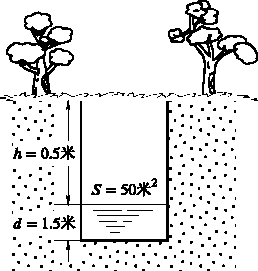
\includegraphics{figure/fig06.15}
  \caption{}
  \label{fig:06.15}
\end{wrapfigure}
\exercise 把一长为$ L $、质量为$ m $平放在地上的细杆竖立起来,另一
端仍在原地,至少要作多少功?

\exercise 如图\ref{fig:06.15}\;所示,一蓄水池面积为$ S = 50 \;\text{米} ^ 2 $,所蓄的水面比地面低5.0米,水深$ d=1.5 $米。
用抽水机把这池里的水全部抽到地面上,至少要作多少功?

\exercise 用水泵抽水,水面低于水
泵喷口$ h _ { 1 } = 2.0 $米;水泵喷口横截面为$ a = 3 0 \;\text{厘米} ^ 2 $,喷口仰角为$
  30 ^ { \circ } $,喷射水流的顶点比喷嘴高出$ h _ { 2 } = 4.0 $米,如图\ref{fig:06.16}\;所示。假
如水泵马达的效率为60\%,忽略空气阻力,输电线供给的功率是
多少?

\begin{figurex}
  \centering
  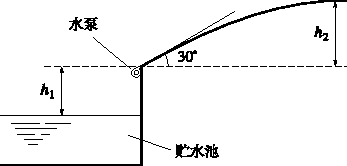
\includegraphics{figure/fig06.16}
  \caption{}
  \label{fig:06.16}
\end{figurex}

\exercise 一物体受到$ F = - 6 x ^ { 3 } $的力的作用,$ x $以米为单位,$ F $以牛
顿为单位。物体从$ x = 1.0 $米移到$ x = 2.0 $米时,力$ F $作了多少功?

% 192.jpg
\clearpage
\exercise 有一缓慢改变倾角的固定斜面,如图\ref{fig:06.17}\;所示,其斜面
与水平部分的摩擦系数都相同。今有一物体从高为处自由下滑,
最后停在离起点的水平距离为$ s $的水平面上。试证: $ \mu = h / s $。
\begin{figurex}
  \centering
  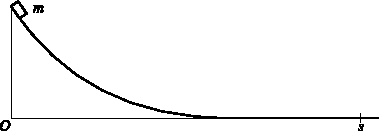
\includegraphics{figure/fig06.17}
  \caption{}
  \label{fig:06.17}
\end{figurex}

\exercise 从功能关系出发,试证明,质量为$ M $的汽车,以速度$ v $沿
水平公路行驶时,要它停下来所需的最短距离为$ v ^ { 2 } / 2 \mu g $($ \mu $为汽车
车轮与路面间的滑动摩擦系数)。

\exercise 长为$ L $、质量为$ m $的一条细铁链,开始时长为$ a $的一段垂
在桌面下,拉住上端使整个铁链静止不动(图\ref{fig:06.18});然后放手让
它滑下。不计摩擦阻力,铁链上端离开桌面时,其下落的速度$ v $
是多少?
\vspace{1.56em}
\begin{figurex}
  \begin{minipage}[b]{0.4\linewidth}
    \centering
    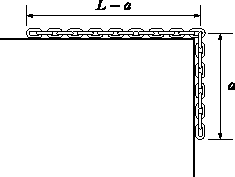
\includegraphics{figure/fig06.18}
    \caption{}
    \label{fig:06.18}
  \end{minipage}
  \hfill
  \begin{minipage}[b]{0.6\linewidth}
    \centering
    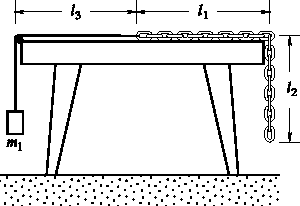
\includegraphics{figure/fig06.19}
    \caption{}
    \label{fig:06.19}
  \end{minipage}
\end{figurex}

\exercise 重10公斤、长40厘米的链条,放在光滑的水平桌面上,其
一端拴一细绳,绳子通过滑轮悬着一个质量$ m _ { 1 } = 10 $公斤的物体
% 193.jpg
(图\ref{fig:06.19})。开始时$ l _ { 1 } = l _ { 2 } = l _ { 3 } = 20 $厘米,系统速度为零。设绳长不
变,绳的质量及绳与滑轮摩擦可不计。当链条全部滑到桌面上
($ l _ { 2 } = l _ { 3 } = 0 $, $ l _ { 1 } = 40 $厘米)时,系统的速度$ v $是多少?

\exercise 质量为$ m = 1.0 $公斤的木块在一水平面上与一倔强系数
$ k = 2.0 $牛顿/米的弹簧发生正碰撞,弹簧另一端是固定的,木块将
弹簧由来静止且自自伸展的位置压缩4.0米(图\ref{fig:06.20})。设木块与
水平面间的滑动摩擦系数为0.25,木块原来的速率$ v _ { 0 } $是多少?
\begin{figurex}
  \begin{minipage}[b]{0.7\linewidth}
    \centering
    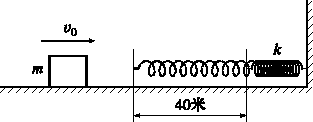
\includegraphics{figure/fig06.20}
    \caption{}
    \label{fig:06.20}
  \end{minipage}
  \hfill
  \begin{minipage}[b]{0.25\linewidth}
    \centering
    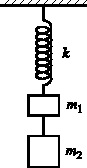
\includegraphics{figure/fig06.21}
    \caption{}
    \label{fig:06.21}
  \end{minipage}
\end{figurex}

\exercise 在倔强系数为$ k $的弹簧下面悬挂质量分别为$ m_1 $及$ m_2 $的物
体,开始时处于静止,如图\ref{fig:06.21}\;所示。若突然割断$ m _ { 1 } $与$ m_2 $间的连
线,试求$ m _ { 1 } $所能达到的最大速度$ V_{\max} $。

\exercise 一物体以初速率$ v _ { 0 } = 14 $ 米/秒由240米高处落入地面上的
沙内,深达0.20米。试求沙对物体所施的平均阻力$ F $(不计空气
阻力)。

\begin{wrapfigure}[7]{r}{17em}
  \centering
  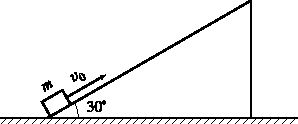
\includegraphics{figure/fig06.22}
  \caption{}
  \label{fig:06.22}
\end{wrapfigure}
\exercise 一个固定斜面倾角$ \alpha = 30 ^ { \circ } $,外面下端
有一100克的小物体,开始时以19.8米/秒的
速率沿斜面向上冲(图\ref{fig:06.22}),走了20米远便停
下来,然后下滑。
% 194.jpg

\clearpage
(1)计算物体起始的动能和在最高点时的势能;

(2)求斜面作用于物体的摩擦力$ f _ { \mu } $;

(3)求物体滑回下端的时间。

\exercise 一个质量为$ m $的质点在一个固定的、半径为$ r $的光滑球面
的顶点,从静止开始下滑,如图\ref{fig:06.23}\;所示。现用图中的角度$ \theta $来
表示质点的位置,选出发点处的势能为零。试求

(1)以$ \theta $为变量的势能函数;

(2)以$ \theta $为变量的动能函数;

(3)以$ \theta $为变量的径向和切向加速度;

(4)质点离开球面时刻的角度。
\vspace{1.56em}
\begin{figurex}
  \begin{minipage}[b]{0.5\linewidth}
    \centering
    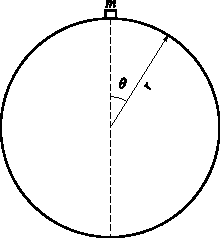
\includegraphics{figure/fig06.23}
    \caption{}
    \label{fig:06.23}
  \end{minipage}
  \hfill
  \begin{minipage}[b]{0.5\linewidth}
    \centering
    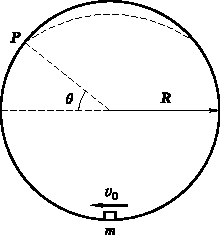
\includegraphics{figure/fig06.24}
    \caption{}
    \label{fig:06.24}
  \end{minipage}
\end{figurex}

\exercise 一质量为$ m $的质点在半径为$ R $的竖直圆轨道内运动,设没
有摩擦力,当质点在最低点时,其速率为$ v_ 0 $,如图\ref{fig:06.24}\;所示。

(1)\;$ v $的最小值$ v _ { \text { min } } $为多大时,质点还能沿着圆形轨道运动而
不脱离轨道?

(2)假定$ v _ { 0 } = 0.775 v _ { \text { min } } $,则质点将在某点$ P $处脱离轨道而沿
图6.24中虚线所示的路径运动,试求$ P $点的角位置。

\exercise 一质量为$ m $的小物体从一下坡轨道的$ A $点由静止出发下
% 195.jpg
滑,下坡轨道的下端接着一个以$ O $点为圆心、半径为$ R $的圆形轨
道。设轨道都在竖直平面内(图\ref{fig:06.25}),$ A $与$ O $的高度差为$ h $,略去
摩擦。求:

(1)它到达圆形轨道最高点$ B $时的速度、它所受的力以及它
作用在轨道上的力$ N _ { B } $;

(2)要使$ m $不离开轨道下落,$ h $至少应为多少?

\vspace{1.56em}
\begin{figurex}
  \begin{minipage}[b]{0.63\linewidth}
    \centering
    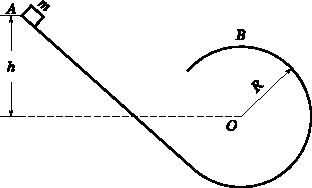
\includegraphics{figure/fig06.25}
    \caption{}
    \label{fig:06.25}
  \end{minipage}
  \begin{minipage}[b]{0.35\linewidth}
    \centering
    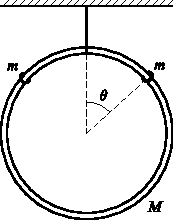
\includegraphics{figure/fig06.26}
    \caption{}
    \label{fig:06.26}
  \end{minipage}
\end{figurex}
\vspace{1.56em}

\exercise 用一条细线把质量为$ M $的圆环挂起来,环上有两个质
为$ m $的小环,它们可以在大环上无摩擦地滑动(图\ref{fig:06.26})。若两个小
环同时从大环顶部释放并沿相反方向自由滑下,试证:如果$ m >
  \dfrac { 3 } { 2 } M $
,则大环在$ m $落到一定的角位置$ \theta $时会升起,求大环开始上
升时的角度$ \theta $。

\exercise (1)一升降机匀速下降,它的吊绳突然被卡住,这时绳内
的张力将怎样变化?

(2)设升降机的质量为$ M = 3.0 $ 吨,原来下降的速度为$ v _ { 0 } =
  1.0 $米/秒,绳子的倔强系数$ k = 1.00 $吨/厘米。试计算上述过程中
绳上的最大张力和相应的伸长量(设整个过程在绳子的弹性限度
内)。

% 196.jpg
\clearpage
\exercise 一质量为$ M $的火车在平直轨道上匀速前进时,最后一节
质量为$ m $的车厢突然脱落,这车厢在走了长的路程后停止。假设
机车的牵引力和列车与轨道间的摩擦系数都不变,当脱落的那节
车厢停止时,列车距此车厢多远?

\exercise 一杂技演员从距网$ h = 1 0 $米高处落到弹性网上。如果演
员站在网上静止不动时,网的弯曲深为$ x _ { 0 } = 2 0 $厘米。问演员从高
处落到网上时对网的最大压力是演员本身重量的多少倍?

\exercise 一均匀球体,半径为$ R $,质量为$ M $。求离中心为处的引
力势能$ U\left(r\right) $(即单位质量的位能),并画出$ U \mathdash r $曲线。

\exercise 求证地球表面上高度为$ h $处的逃逸速度为
\begin{equation*}
  v = v _ { 2 } \sqrt { \frac { R } { R + h } }
\end{equation*}
式中$ R $是地球半径,$ v _ { 2 } $是地球表面上的逃逸速度。

\exercise 在一半径为$ R_0 $的无空气的小行星表面上,若以速率$ v_0 $水
平地抛出一物体,则该物体恰好环绕该行星的表面作匀速圆周运
动。问:

(1)这小行星的逃逸速度是多少?

(2)在这星体表面竖直上抛一物体,要使它达到$ R_0 $的最大高
度,上抛速率是多少?若要使该物体达到$
  \dfrac { 1 } { 2 } R_0 $的高度,上抛速
率又应是多少?

(3)一质量为$ m $的物体,在离该星表面上高度为$ y \left( y < R _ { 0 } \right) $
处,它的位能是多少?\lhbrak 展成$ y / R _ { 0 } $的级数,保留到$ \left( y / R _ { 0 } \right) ^ { 2 } $项。\rhbrak

(4)如果$ y \ll R _ { 0 } $,要使物体从行星表面升到$ y $的高度,它的上
抛速率至少为多少?\lhbrak 与(3)一样作近似,保留到$ \left( y / R _ { 0 } \right) ^ { 2 } $项。\rhbrak

\exercise 质量为$ m $和$ M $的两个质点最初处于静止态状并相距无穷
远,试证:由于引力作用,它们在任何时刻互相趋近的相对速度为
$ \sqrt { 2 G \left( M + m \right) / d } $。这里$ d $是在该时刻两质点间的距离。

% 197.jpg
\exercise 两个质量均为1.0克的质点,相距10米。开始时相对静止,
如果它们之间只有引力作用,它们何时相碰?

\exercise (1)无穷远处的流星相对地球中心的速度很小,它在地
球引力作用下落到地面,若不计空气阻力,试问:它将以多大的
速度落到地球表面。

(2)实际上,阻力不可忽略。设只有径向运动,且阻力数值与
速度成正比,试列出其运动方程。

(3)下雨的过程都发生在对流层,在这区间,重力加速度$ g $可认
为是常数。试问:一个质量为$ m $的雨滴将以怎样的速度落到地面?

32.地震的里氏(Richter)震级公式为:
$ \log E _ { M } = 12.24 + 1.44 M $
式中$ E _ { M } $是某次地震释放出的能量(以尔格计);$ M $是该次地震的震
级。清康熙十八年七月廿八日(公元1679年9月2日),北京地区发
生过一次八级地震($ M = 8 $) 。试问:

(1)该次地震释放的能量是多少?

(2)如果用此能量把重物从地面上举起,它能把多少质量的
物体升高1公里?

\exercise 根据最新勘测资料,我国长江的长度居世界第三,它的主
源头是青海高原昆仑山南麓的托托河,从这里经5,000米落差注入
东海,它的水利资源的储藏量是$ 1.125 \times 10 ^ { 8 } $千瓦。据此计算长江
的平均流量。

\end{exercises}